% !TEX encoding = UTF-8
% !TEX program = pdflatex

% This is "sig-alternate.tex" V2.0 May 2012
% This file should be compiled with V2.5 of "sig-alternate.cls" May 2012
%
% This example file demonstrates the use of the 'sig-alternate.cls'
% V2.5 LaTeX2e document class file. It is for those submitting
% articles to ACM Conference Proceedings WHO DO NOT WISH TO
% STRICTLY ADHERE TO THE SIGS (PUBS-BOARD-ENDORSED) STYLE.
% The 'sig-alternate.cls' file will produce a similar-looking,
% albeit, 'tighter' paper resulting in, invariably, fewer pages.
%
% ----------------------------------------------------------------------------------------------------------------
% This .tex file (and associated .cls V2.5) produces:
%       1) The Permission Statement
%       2) The Conference (location) Info information
%       3) The Copyright Line with ACM data
%       4) NO page numbers
%
% as against the acm_proc_article-sp.cls file which
% DOES NOT produce 1) thru' 3) above.
%
% Using 'sig-alternate.cls' you have control, however, from within
% the source .tex file, over both the CopyrightYear
% (defaulted to 200X) and the ACM Copyright Data
% (defaulted to X-XXXXX-XX-X/XX/XX).
% e.g.
% \CopyrightYear{2007} will cause 2007 to appear in the copyright line.
% \crdata{0-12345-67-8/90/12} will cause 0-12345-67-8/90/12 to appear in the copyright line.
%
% ---------------------------------------------------------------------------------------------------------------
% This .tex source is an example which *does* use
% the .bib file (from which the .bbl file % is produced).
% REMEMBER HOWEVER: After having produced the .bbl file,
% and prior to final submission, you *NEED* to 'insert'
% your .bbl file into your source .tex file so as to provide
% ONE 'self-contained' source file.
%
% ================= IF YOU HAVE QUESTIONS =======================
% Questions regarding the SIGS styles, SIGS policies and
% procedures, Conferences etc. should be sent to
% Adrienne Griscti (griscti@acm.org)
%
% Technical questions _only_ to
% Gerald Murray (murray@hq.acm.org)
% ===============================================================
%
% For tracking purposes - this is V2.0 - May 2012

\documentclass{sig-alternate}
\usepackage[utf8]{inputenc}
\usepackage{listings}
\usepackage{url}
\usepackage{footnote}
\usepackage{color}
\usepackage{colortbl}%
  \newcommand{\myrowcolour}{\rowcolor[gray]{0.925}}
\usepackage{xcolor}

\newcommand{\ie}{{\em i.e.,~}}
\newcommand{\eg}{{\em e.g.,~}}
\newcommand{\etc}{{\em etc}}

\lstdefinelanguage{Scala}%
{morekeywords={abstract,case,catch,char,class,%
    def,else,extends,final,%
    if,import,%
    match,module,new,null,object,override,package,private,protected,%
    public,return,super,this,throw,trait,try,type,val,var,with,implicit,%
    macro,sealed,%
  },%
  sensitive,%
  morecomment=[l]//,%
  morecomment=[s]{/*}{*/},%
  morestring=[b]",%
  morestring=[b]',%
  showstringspaces=false%
}[keywords,comments,strings]%

\lstset{tabsize=2,
basicstyle=\ttfamily\fontsize{7pt}{1em}\selectfont,
commentstyle=\itshape\rmfamily,
numbers=left, numberstyle=\scriptsize\color{gray}\ttfamily, language=scala,moredelim=[il][\sffamily]{?},mathescape=false,showspaces=false,showstringspaces=false,xleftmargin=15pt,escapechar=@, morekeywords=[1]{let,fn,val},deletekeywords={for},classoffset=0,belowskip=\smallskipamount
}

\begin{document}
%
% --- Author Metadata here ---
\conferenceinfo{AGERE!}{'15 Pittsburgh, Pennsylvania, USA}
%\CopyrightYear{2007} % Allows default copyright year (20XX) to be over-ridden - IF NEED BE.
%\crdata{0-12345-67-8/90/01}  % Allows default copyright data (0-89791-88-6/97/05) to be over-ridden - IF NEED BE.
% --- End of Author Metadata ---

% \title{Towards a portable actor runtime environment}
\title{Akka.js: Towards a portable actor runtime environment}

%
% You need the command \numberofauthors to handle the 'placement
% and alignment' of the authors beneath the title.
%
% For aesthetic reasons, we recommend 'three authors at a time'
% i.e. three 'name/affiliation blocks' be placed beneath the title.
%
% NOTE: You are NOT restricted in how many 'rows' of
% "name/affiliations" may appear. We just ask that you restrict
% the number of 'columns' to three.
%
% Because of the available 'opening page real-estate'
% we ask you to refrain from putting more than six authors
% (two rows with three columns) beneath the article title.
% More than six makes the first-page appear very cluttered indeed.
%
% Use the \alignauthor commands to handle the names
% and affiliations for an 'aesthetic maximum' of six authors.
% Add names, affiliations, addresses for
% the seventh etc. author(s) as the argument for the
% \additionalauthors command.
% These 'additional authors' will be output/set for you
% without further effort on your part as the last section in
% the body of your article BEFORE References or any Appendices.

\numberofauthors{3} %  in this sample file, there are a *total*
% of EIGHT authors. SIX appear on the 'first-page' (for formatting
% reasons) and the remaining two appear in the \additionalauthors section.
%
\author{
% You can go ahead and credit any number of authors here,
% e.g. one 'row of three' or two rows (consisting of one row of three
% and a second row of one, two or three).
%
% The command \alignauthor (no curly braces needed) should
% precede each author name, affiliation/snail-mail address and
% e-mail address. Additionally, tag each line of
% affiliation/address with \affaddr, and tag the
% e-mail address with \email.
%
% 1st. author
\alignauthor
Gianluca Stivan\\
       \affaddr{UniCredit R\&D}\\
       \affaddr{Italy}\\
       \email{Gianluca.Stivan@stud-inf.unibz.it}
% 2nd. author
\alignauthor
Andrea Peruffo\\
       \affaddr{UniCredit R\&D}\\
       \affaddr{Italy}\\
       \email{Andrea.Peruffo@unicredit.eu}
% 3rd. author
\alignauthor Philipp Haller\\
       \affaddr{KTH Royal Institute of Technology}\\
       \affaddr{Sweden}\\
       \email{phaller@kth.se}
\and  % use '\and' if you need 'another row' of author names
% 4th. author
% \alignauthor Lawrence P. Leipuner\\
%        \affaddr{Brookhaven Laboratories}\\
%        \affaddr{Brookhaven National Lab}\\
%        \affaddr{P.O. Box 5000}\\
%        \email{lleipuner@researchlabs.org}
}

\maketitle
\begin{abstract}
Multiple mature implementations of the actor model of concurrency exist. Besides several ones available for the Java Virtual Machine, there are others, for example, written in SmallTalk or in C++, targeting native platforms or other virtual machines. Recently, runtime environments for platforms such as GPUs have also appeared.

However, so far, no full-featured actor runtime environment has allowed actor programs to run, unchanged, on both Java and JavaScript virtual machines. This paper describes our ongoing effort in providing a portable implementation of the widely-used Akka actor framework.
\end{abstract}

% A category with the (minimum) three required fields
% \category{H.4}{Information Systems Applications}{Miscellaneous}
%A category including the fourth, optional field follows...
% \category{D.2.8}{Software Engineering}{Metrics}[complexity measures, performance measures]

% \terms{Theory}

\keywords{Actors, Portability, Akka, Scala, Java, JavaScript}

\section{Introduction}
Since its introduction in 1995~\cite{web:js} there has been an increasing interest in JavaScript. Originally, this programming language was developed by Netscape to provide a lightweight interpreted language to attract non-professional programmers. Later on, thanks to a standardization process started in 1996 and still continuing today with the release of the sixth version in June 2015~\cite{web:ecmascript6}, JavaScript has become the most popular programming language on the web, and is widely regarded as the assembler of the web.

It is interesting to analyze the evolution of the language. Before the introduction of Ajax~\cite{web:ajax} JavaScript was mainly used for simple scripting tasks in the browser. In 2009 CommonJS~\cite{web:commonjs} and Node.js~\cite{web:nodejs} proposed an ecosystem capable of running\newline JavaScript outside the browser. With the rise of single-page web applications~\cite{web:spa} and source-to-source compilers~\cite{web:compile2js}, this once very limited language is now being used to power a large variety of projects.

Despite the improvements made by the JavaScript community, there are still several issues that make developing software using JavaScript hard, which is why it is commonly considered inconvenient to work with. Since it was born as a scripting language there are a number of questionable points:

\begin{itemize}
	\item[-] it did not provide a module system up to ES6~\cite{web:es6modules};
	\item[-] it is weakly and dynamically typed;
	\item[-] the syntax for function definition is verbose;\footnote{Even if JavaScript's support for closures is commonly noted as being one of its\rq{s} redeeming features.}
	\item[-] late binding has poor guarantees;\footnote{Early binding allows for static verification of the existence of method-signature pairs.}
	\item[-] the behavior of \emph{this};
	\item[-] implicit casting, which not always has desired consequences.
\end{itemize}

The biggest issue that JavaScript has, though, is its almost complete lack of support for concurrency. As a language that is by default asynchronous, since all I/O is done via event-based APIs, it is surprising that the only way to write asynchronous code is through callbacks (up to ES6) and promises~\cite{LiskovS88} (from ES6 upwards). This quickly leads to a loss of the application flow due to the difficult way of managing callbacks' composition because inversion of control, i.e., it suffers from deeply-nested functions, is prominent.

The actor model~\cite{Hewitt77,Agha} has been successfully used to write concurrent and distributed applications in a variety of domains, ranging from telephone switches~\cite{ErlangApplications}, to critical infrastructure services written in Erlang~\cite{Armstrong10} such as Amazon's S3 and so on. As such the model would be a perfect fit for JavaScript, but unfortunately there is no widely used or supported implementation of such a model that targets JavaScript runtimes.

After evaluating different virtual machine environments, we found in Akka~\cite{Akka} a mature actor framework for the JVM~\cite{Lindholm-Yellin}, which can be used both from Scala~\cite{OderskyR14} and from Java. Given the existence of Scala.js~\cite{Scalajs}, a\newline Scala-to-JavaScript compiler, we started investigating the feasibility of porting said Akka framework to JavaScript. Unfortunately, as the framework is written today, it is heavily dependent on the JVM.

Specifically, this paper presents our ongoing effort to enable {\em portability} of systems and applications based on actors in Scala~\cite{ActorsInScala}, using the Akka actor-based middleware. Traditionally, actor-based programs in Scala have been restricted to run on the JVM, Scala's main compilation target.

We argued that the actor model is beneficial to JavaScript, but why? Enabling actor-based applications to be deployed on JavaScript runtimes presents numerous advantages. To begin with, it brings an arguably very good model, which handles concurrency and fault handling admirably, to a runtime which lacks good support for both. Moreover, it promotes state isolation, which simplifies reasoning about application code. Finally, the message passing abstraction fits incredibly well to a variety of I/O operations that JavaScript provides. WebSockets, WebWorkers, AJAX, and DOM\newline events are all asynchronous and event-based, making a wrapper that forwards events as messages to actors at the same time convenient and simple to use.

\subsection{Contributions}

{\em Akka.js}\footnote{See \url{https://github.com/unicredit/akka.js}} is our solution to the problem of providing a fully-featured Scala actor framework for JavaScript runtimes (ES5 and above). It enables portable actor-based applications, compiled against the Akka API, to target both the JVM and JavaScript runtimes. Another important goal of the project is seamless messaging between actors running on JavaScript runtimes (\eg web browsers) and actors running on JVMs.

More specifically, our approach can be divided into the following contributions:
\begin{itemize}
	\item[-] Porting the original JVM-based implementation of\newline Akka (from now on referred to as Akka.JVM) to\newline JavaScript;
	\item[-] Techniques for sharing Scala code between Akka.JVM and Akka.js;
       \item[-] An approach for enabling transparent interoperability between actors running on JavaScript runtimes and actors running on JVMs.
\end{itemize}
\noindent
The second issue is of major importance: the lack of a shared code base would require {\em manual synchronization} between two large code bases, with a corresponding large engineering cost. Moreover, the lack of automatic, compile-time checks would make it extremely difficult to ensure the portability of Akka-based programs across Akka.JVM and Akka.js in the long run.

The paper proceeds as follows. We first give a brief\newline overview of the Scala.js compiler, the Akka actor framework, as well as a previous prototype of an actor system for Scala.js (\S~\ref{sec:background}). We then discuss the major challenges encountered during the development of Akka.js (\S~\ref{sec:challenges}), which include reliance on JVM constructs (data structures, patterns, and libraries), usage of reflection, blocking APIs, and serialization. We also detail the solutions adopted to circumvent the presented issues. After that, we outline a number of potential use cases for Akka.js (\S~\ref{sec:usecases}). Finally, following a discussion of related work (\S~\ref{sec:related}), we offer an outlook and conclude (\S~\ref{sec:conclusion}).

\section{Background}\label{sec:background}

\subsection{Scala.js}

Scala.js is an alternative compiler for the Scala language that instead of targeting the Java Virtual Machine's bytecode, targets JavaScript.
As many other efforts in and out the JVM (GWT, CoffeeScript, ...) the goal of the project is to provide a language which is higher-level than JavaScript, in order to achieve easier code reusability and to provide better abstractions and tooling.
One key point of Scala.js, and crucial to the topic of this paper, is bi-directional JavaScript interoperability, meaning that plain JavaScript libraries can be wrapped by Scala interfaces and used in Scala.js and Scala.js can expose user-defined APIs to JavaScript.
The project actually features a 100\% coverage of the Scala language  (apart from few intentional differences due to semantics) and has got a lot of useful facades to the most popular JavaScript libraries,
Since most of the to-JavaScript compilers suffer from performance penalties, it is important to note that fully optimized Scala.js code executes at almost native JavaScript speed.


\subsection{Akka}\label{sec:akka}

Akka~\cite{Akka} is a library written for the Java Virtual Machine which enables programmers to write scalable, resilient, and responsive applications. It does so by providing a high-level abstraction built on top of the actor model and, although written in Scala, it can be used from other JVM-based languages as well.

Akka was originally created by Jonas Bon\'{e}r, and has since evolved to provide all kinds of abstractions over actors. It is also included by default in the Scala standard library.

Akka provides a number of advantages:
\begin{itemize}
  \item[-] Simple and high-level abstractions for concurrency and parallelism.
  \item[-] Asynchronous, non-blocking and highly-performant\newline event-driven programming model.
  \item[-] Very lightweight event-driven processes (several million actors per GB of heap memory).
  \item[-] Fault tolerance through supervisor hierarchies with ``let-it-crash'' semantics.
  \item[-] Location transparency in distributed environments,\newline pure asynchronous message passing.
\end{itemize}

Thus, both aspects of the actor model are covered, (a) an API that supports writing concurrent software using the abstraction provided by actors, and (b) a runtime library that provides powerful features for error handling and actor life-cycle management.

Moreover, Akka seamlessly integrates the actor model into the unified object-oriented and functional programming style that Scala enables~\cite{OderskyR14}. Techniques for integrating actors into Scala have been explored in the context of Akka's predecessor, Scala Actors~\cite{HallerO09}.

To introduce Akka's programming model, we look at its components, first of all the ActorSystem, which is the very first element you interact with, when using this library.
An ActorSystem is a high-level abstraction over a container of actors; it is heavyweight and wraps a thread pool to abstract the underlying, JVM-specific concurrency model.
All actors must be spawned within an ActorSystem. By creating several ActorSystems, it is possible to separate different runtime requirements even within the same JVM process.
Creating a new ActorSystem is dead simple:
\begin{lstlisting}
val system = ActorSystem.create
\end{lstlisting}
\noindent
Akka actors are containers for state, behavior, a mailbox, children, and a supervision strategy. The detached interface that enables the interaction with the rest of the world is represented by an ActorRef, short for actor reference.
Akka provides a special Actor trait\footnote{Scala supports a safe form of multiple inheritance through modular mix-in composition of traits. Traits in Scala can be thought of as more flexible Java interfaces.} with concrete and abstract members that can be extended by any arbitrary subclass.
In this case, the only abstract member that subclasses have to define in order to create a concrete instance of an actor is the \verb|receive| method:
\begin{lstlisting}
def receive: PartialFunction[Any, Unit]
\end{lstlisting}
\noindent
Method \verb|receive| returns a partial function which is synchronously applied to each message that is dequeued from the actor's mailbox. Messages are automatically processed one by one as long as the mailbox is not empty.

A common practice in Scala is to use {\em pattern matching} to destructure the messages an actor receives. The following simple actor prints a message to the console when it receives the string ``ping.''
\begin{lstlisting}
class PingReceiver extends Actor {
  def receive = {
    case "ping" => println("Ping message received")
  }
}
\end{lstlisting}
\noindent
Since actor objects have specific properties (\eg their state is fully encapsulated), they cannot be instantiated using regular means. A previously-created ActorSystem enables spawning new actors within itself using the so-called ``Prop'' objects. A Prop object is a container of (actor) creation properties which specifies various runtime configuration properties (the discussion of which is outside the scope of this short overview). At the minimum, an \verb|Actor|-extending class containing the actor's behavior must be specified:
\begin{lstlisting}
val actor = system.actorOf(Props[PingReceiver])
\end{lstlisting}
\noindent
In order to send messages to the spawned actor, the usual \verb|!| operator is used:
\begin{lstlisting}
actor ! "ping"
\end{lstlisting}
\noindent
In this case, the expected result, ``Ping message received'', is printed to the console.

Akka not only provides what was covered in this brief overview, but a rich toolkit for creating distributed actor-based systems on elastic cloud computing platforms as well.


\subsection{Scala.js Actors}

The original source of inspiration for Akka.js was \textit{Scala-js-actors}.
Developed as a semester project by EPFL PhD student Sébastien Doeraene in fall 2013, it was designed as a way to prove Scala-js' real world capabilities.
The code contains a small subset of the entire Akka.JVM codebase, but already has support for actors, supervision and fault-tolerancy.
Scala-js-actors was further extended to provide interoperability with an Akka.JVM backend through WebSockets and multi-core computation using WebWorkers.


While an amazing piece of engineering, the limits of scala-js-actors are:
\begin{itemize}
\item[-] No strong relationship with the original Akka codebase;
\item[-] No testing suite;
\item[-] Different semantics from Akka.JVM remote, the Akka module for communicating with remote nodes.
\end{itemize}
To elaborate a bit further, the first two points where due to the fact that scala-js-actors was a research project, a proof of concept of the maturity of Scala.js, hence it was not designed with a long-term strategy in mind.
The third point is more vital. Akka.JVM remote is the component that allows different JVMs to seamlessly communicate between them using the same abstraction that one would use for local actors. It's the ultimate implementation of the location transparency concept of the actor model.
Whereas in Akka.JVM the programmer needs only to configure the cluster and there is no perceivable difference between
remote and local actors:
\begin{lstlisting}
localActor ! "msg"
remoteActor ! "msg"
\end{lstlisting}
In scala-js-actors configuration is not supported, meaning that the programmer has to take care of the setup
\begin{lstlisting}
// Main
...
WebWorkerRouter.initializeAsRoot()
val workerAddress =
  WebWorkerRouter
    .createChild("worker.js")
// Child
...
WebWorkerRouter.setupAsChild()
WebWorkerRouter.onInitialized { ... }
\end{lstlisting}
In the above example, \emph{WebWorkerRouter} is necessary because it takes care of routing the messages to the
correct actor, since there is no underlying platform that takes care of it, as it is the case with Akka.JVM remote.
This poses serious problems when it comes to Akka.JVM interoperability, so for these reasons, it was decided
that it would be beneficial to iterate on the original scala-js-actors codebase and provide a library that
diverges as little as possible from the original Akka, so that it would be instant or trivial to port Akka
applications to the browser.
In particular the benefits Akka.js addresses the 3 main concerns about scala-js-actors by providing a
test suite, a 1-1 ratio with Akka.JVM code and includes in the roadmap full support for akka-remote
semantics.

\section{Portable runtime environment}\label{sec:challenges}

In order to achieve a perfectly portable runtime environment, it is first necessary to understand the semantics of the target.
JavaScript can run in many different environments, including
\begin{itemize}
\item[-]{Node.js, a JavaScript runtime for server side applications;}
\item[-]{Phantom.js, a headless, programmable WebKit browser;}
\item[-]{Rhino, a JavaScript engine running on the JVM;}
\item[-]{Browsers, in general.}
\end{itemize}
These environments, albeit not identical, share some common traits, which simplify the process of understanding where to focus the porting effort. One such trait is the \textit{JavaScript's execution model}.

\subsection{JavaScript's execution model}

JavaScript is, as we briefly mentioned, a dynamic, single-threaded programming language. It provides some functional concepts such as closures and partial support for operating on collections (\eg map, reduce, filter).
JavaScript is also inherently concurrent, since all its I/O operations are asynchronous and event based.
In order to better understand how this affects the development of programs, it is necessary to explicitly specify what we mean when we say \textit{asynchronous event-based I/O}.

JavaScript only has a few ways of interacting with the outside world: one is the Document Object Model, a tree-like structure which represents the HTML of the current web page, another is WebSockets and all the AJAX family which include facilities to communicate with a remote server, and finally there is WebWorkers, a novel standard which allows multiple JavaScript runtimes to be spawned and communicate with one another through message passing.
Every time we interact with one of these components a return value isn't immediately available, but the programmer must register explicit interest in the appropriate event. This is where the event loop comes into play. This event loop is a regular loop which listens for events and subsequentially executes the corresponding handler that the programmer has specified, using a callback mechanism.

\subsection{Akka.js}

Akka.js is the core project of this paper, and as previously mentioned, builds on \textit{scala-js-actor}. The original codebase has been pretty much rewritten from scratch to more closely mimic the Akka.JVM code, but Doeraene's work has served as a great source of inspiration.
What Akka.js really is, is a partial port of the Akka ecosystem to Scala.js, which allows Akka programs to run directly everywhere JavaScript is available. It achieves this by replacing all the Java Virtual Machines dependencies with their JavaScript counterparts while keeping the semantics of the library unchanged. The project provided some interesting challenges, some of which are mentioned below.

\subsubsection{Challenge 1: JVM dependency}

The biggest problem that arose was the heavy dependency on JVM code that Akka.JVM has. JVM code is intertwined with code that can be shared with Akka.JS and there is no easy way to remove it. Examples of such dependency are threads, JVM data structures and JS semantics differing from the JVM.
The problem was solved in two ways. First, code was divided in two directories, one with JavaScript specific code, another with code that is shared with Akka.JVM. Second, the JavaScript specific code was rewritten from scratch to allow Akka to run in JavaScript runtimes with the same semantics as in the Java Virtual Machine.

\subsubsection{Challenge 2: JVM-style reflection}

A further problem which was encountered during the development of Akka.js was due to the reflection usage on the JVM. Reflection is a feature of the Java SDK which allows a programmer to inspect an object at runtime and interact with it in ways that would not normally be possible. Unfortunately, support for such features is non-existent in the JavaScript runtime, so it was necessary to develop a custom solution. A subset of the \emph{java.lang.reflect} APIs was developed, which is semantically identical to the JVM counterparts. A proposal has also been submitted to the Scala.js core team, to allow for a tighter integration with the compiler.
If the proposal is accepted, this will result in a superior kind of integration and it will be possible to definitely eliminate the last hacky bits in the code.

\subsubsection{Challenge 3: blocking APIs}

Finally, the usage of JVM's blocking APIs in the test code has proven to be a source of difficulties. Given its single threaded nature, it is not normally possible to block in a JavaScript runtime, effectively rendering the available Akka test code unusable. The limitation was circumvented by writing a custom event loop dispatcher that allows for blocking operations. Normally this would result
in a deadlock, but given the asynchronous nature of Akka, the only blocking code is the test itself, so it ends up working just fine.

\subsection{Cross compilation}\label{sec:cross-compilation}

As long as the Akka project remains very active, we face the problem of a divergent code base and it has been so since the very first versions of Akka.js.
The analysis of the key differences highlighted the following major conflicts:
\begin{itemize}
	\item[-] Semantic differences between components usable in a JavaScript environment;
	\item[-] Java API, which is partially implemented in Java and we cannot support;
	\item[-] Missing annotations vital to expose functionalities to the JavaScript runtime;
	\item[-] A tiny number of small hacks used to keep the developer API clean and simple (mostly reflection-based);
	\item[-] Java data structures.
\end{itemize}
Considering the advantages of having a project that can be compiled reusing a large part of the original code, it was decided to adopt some strategies in order to follow a strategy of ``non-intrusive'' patching as much as possible, for as many source files as possible.
\\
In a file where implementations do not conform to the semantics of the JavaScript Virtual Machines, the implementations and interfaces are split in different files, so that Akka.js only depends on the interfaces. The changes are then forwarded to the upstream Akka repository by means of a Pull Request.
Since the Java API is hard-wired directly into the interfaces, the current solution drops the methods at compile time via a compiler plugin.
The same solution, using a compiler plugin, is also adopted to add Scala.js annotations at compile time, where required, through AST manipulation.
By analyzing the data structures used in Akka's codebase, we must keep in mind that:
\begin{itemize}
	\item[-] Akka was developed with JVM, concurrency and performances in mind.
	\item[-] The standard Scala collections library was designed to provide an excellent developer experience and a consistent fully functional API across different kinds of collections, despite possibly worse performance.
\end{itemize}
The obvious conclusion is that the collections that Akka employs are, for said performance reasons, those extremely efficient ones provided by the Java standard library.
When the porting started, the interoperability between the Java standard library and Scala.js was limited to a subset functions concerning Array manipulation.
Instead of chaging the data structures inside Akka itself, to further our goal of compatibility, Scala.js' support of Java collections was extended.
Since JavaScript is single-threaded and asynchronous, there was no need to worry about supporting concurrency safe data structures as this property is intrinsically provided by the runtime.
Collections were therefore implemented through binding on pure Scala data structures and developed respecting pedantically the documentation(JavaDocs) of the JDK.
This resulted in an extensive improvement of the Scala.js/Java inter-compatibility layer that by default ships as part of the compiler.
Today, all Java data structures used by Akka are available in the Scala.js library with the exception of the ``thread-blocking'' ones which would totally compromise the functionality of Akka.js and are, on a JavaScript runtime, therefore not meaningful.


\subsection{Serialization}\label{sec:serialization}

Serialization is essential for {\em remoting}; more specifically, for
communicating messages (a) between different
JavaScript WebWorkers, and (b) between actors running on a JavaScript
runtime (using Akka.js) and actors running on a JVM (using Akka.JVM).
In Akka.JVM, serialization is provided by the underlying virtual
machine--any object can be serialized automatically if its class is
marked as ``serializable'' and all referenced objects are
transitively serializable~\cite{Philippsen2000,Maassen1999}.

It turns out this reliance on the JVM for serialization is a challenge for
Akka.js: contrary to approaches like GWT, Scala.js does not emulate JVM
runtime services like serialization. Moreover, Scala.js does not support
runtime reflection in order to enable important compile-time optimizations
that improve runtime performance and reduce the resulting JavaScript output. Therefore,
using Scala.js it is impossible to implement {\em universal serialization} (as
provided by the JVM) using runtime reflection.

Serialization is also critical for {\em interoperability} between JavaScript
runtimes and JVMs. In particular, an important goal of Akka.js is the
ability to send objects as asynchronous messages between the JavaScript
and the JVM world. Consequently, objects must be serialized in a compatible
way.

\subsubsection{Approach}

Our approach to JavaScript-JVM compatibility is based on generating {\em pickling
combinators}~\cite{MillerHBO13}. Compatibility is achieved through a combination of two
techniques:\footnote{At the time of writing, our implementation is a work-in-progress.
Integration with one of the next major releases of Scala Pickling is planned (see
\url{https://github.com/scala/pickling}).}
\begin{itemize}
\item[-] Serialization is based on a platform-independent external representation.
\item[-] Generated serializers (or {\em picklers}) are cross compiled; as a result,
         serialization on JavaScript runtimes has the same semantics as on the JVM.
\end{itemize}

In order to avoid additional boilerplate compared to\newline Akka.JVM, we are exploring
the use of a Scala compiler plug-in to detect declarations of classes
marked as serializable. For such classes, cross-platform picklers are generated
and automatically registered with the serialization subsystem of Akka.js.
This approach does not require source code changes, at the cost of a minor addition
to the build process.

What is noteworthy about our approach is the fact that we extend an existing,
well-known serialization framework, instead of adopting a custom solution just
for Akka.js. Thus, the developed portability and cross-compilation features benefit other
libraries requiring serialization, such as RPC frameworks. This is similar to
our extensions to Scala.js (see \S~\ref{sec:cross-compilation}), which benefit
a wide range of projects.


\section{Use cases}\label{sec:usecases}

There are many potential uses cases which demonstrate why Akka.js can be extremely beneficial, introducing a new way of thinking about interaction in JavaScript environments. The following examples illustrate potential scenarios where such a library could be successfully employed.

\begin{figure}
\centering
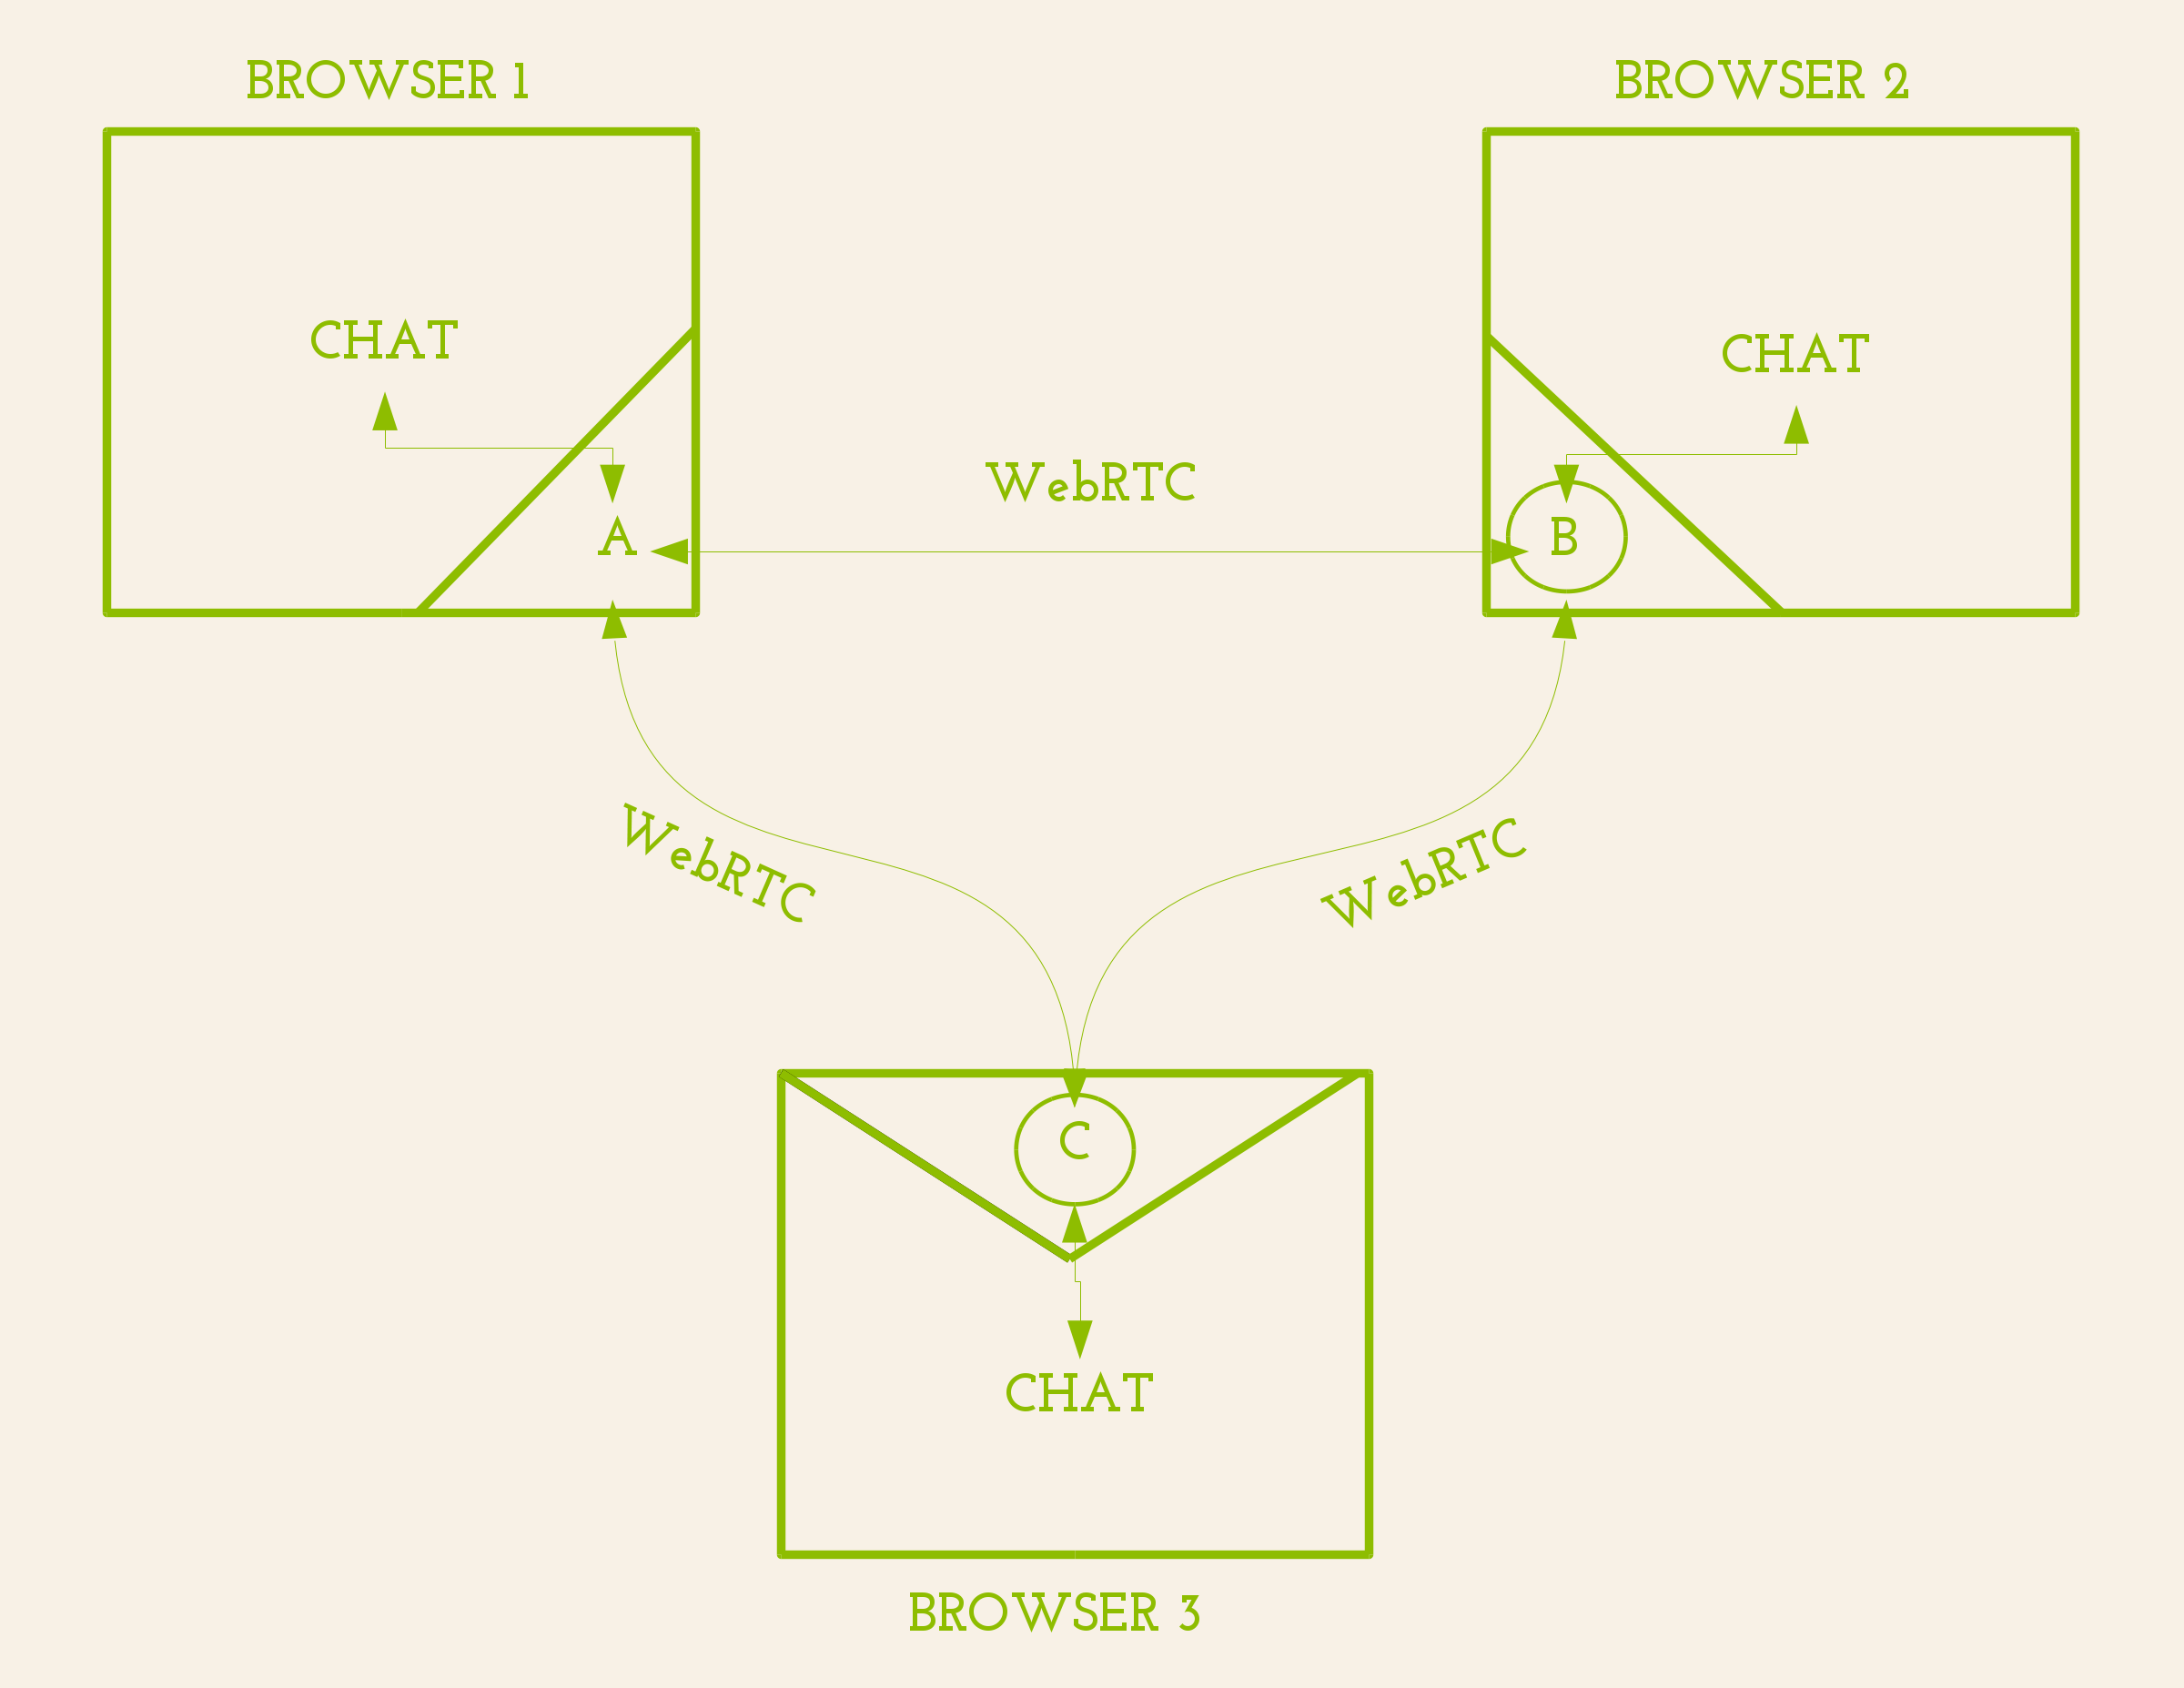
\includegraphics[scale=0.2]{1.png}
\caption{Remoting}
\label{fig:remoting}
\end{figure}

In Figure~\ref{fig:remoting}, a distributed application can be devised using WebRTC as a transport layer.
WebRTC is a technology that allows applications to exploit the benefits of peer-to-peer, from inside
the browser. Given that Akka.js has built-in routing and works by message passing, it would be
possible to abstract away all the complexity from WebRTC and present to the programmer a cluster of
actors which appears local, but instead is running in the nodes of a peer-to-peer network.

\begin{figure}
\centering
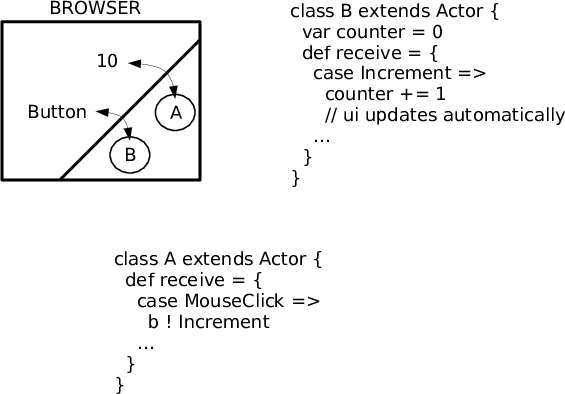
\includegraphics[scale=0.2]{2.png}
\caption{UI Framework}
\label{fig:ui}
\end{figure}

In Figure~\ref{fig:ui}, a new user interface framework could be developed by exploiting the event-driven
architecture of the browser. All user interactions in the browser happen through \emph{events}
which can be handled by the programmer. These events could be wrapped and sent to actors as messages,
transforming all the interactions into one single actor system.

\begin{figure}
\centering
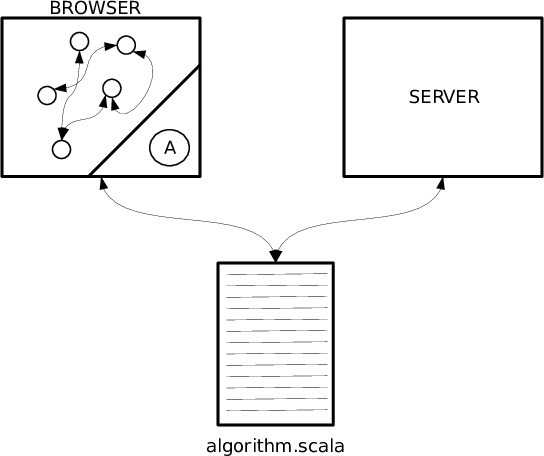
\includegraphics[scale=0.3]{3.png}
\caption{Algorithm visualization}
\label{fig:algorithm}
\end{figure}

The third example in Figure~\ref{fig:algorithm} is potentially interesting for didactic purposes.
It is often difficult to picture exactly how an algorithm works just by looking at a particular implementation.
Many algorithms are also implemented
in Akka.JVM, so it would be interesting to insert some barriers into the algorithm which update a
GUI showing the step-by-step inner workings of the code.

\begin{figure}
\centering
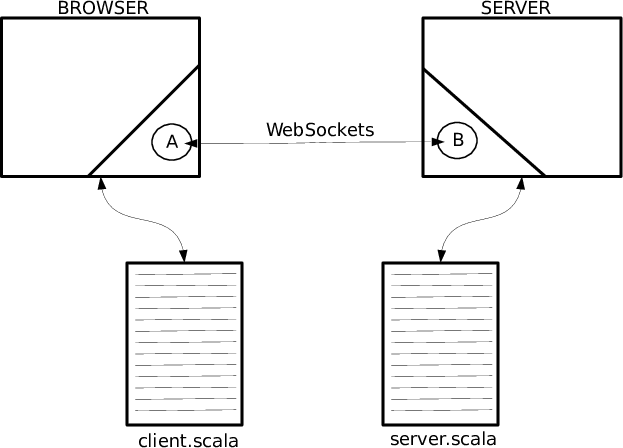
\includegraphics[scale=0.3]{4.png}
\caption{Bi-Directional communication}
\label{fig:communication}
\end{figure}

This fourth example in Figure~\ref{fig:communication} depicts a bi-directional communication channel. Akka.js serves really well as an abstraction layer
that can unite all the different communication protocols. In this case, a frontend application written in Akka.js
can seamlessly interact with a JVM backend running Akka.JVM. The advantage is a unique approach to coding and
the benefit of needing to master only one language, instead of continuously switching from JavaScript to Scala/Java.

\begin{figure}
\centering
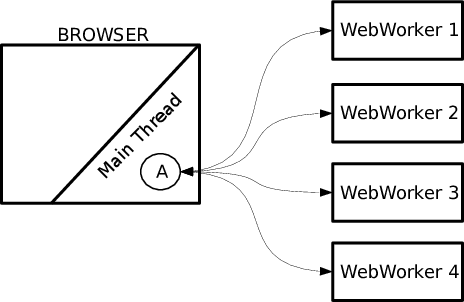
\includegraphics[scale=0.3]{5.png}
\caption{WebWorkers}
\label{fig:ww}
\end{figure}

In the final Figure~\ref{fig:ww}, Akka.js abstracts away the complexity of dealing with WebWorkers. As mentioned before, WebWorkers are a set of API enabling the use of multi-cores in the browser. Unfortunately, because it is only possible to interact with WebWorkers through message passing, it is usually less than trivial to manage everything with JavaScript and a programmer needs to worry about serializing and deserializing messages. Akka.js simplifies the approach, in the sense that the programmer can use the architecture they are already familiar with and Akka.js automatically deals with the low-level components of the WebWorkers without exposing any of its complexity.


\section{Related work}\label{sec:related}

The Clojure language~\cite{Halloway09} supports CSP-style programming~\cite{Hoare78} using its
core.async library. This library is also supported by
ClojureScript~\cite{ClojureScript}, a compiler for Clojure that targets
JavaScript. The main difference in comparison to our effort is the fact that core.async implements the CSP model, whereas Akka.js implements the actor model. CSP also does not directly support distributed computation, meaning that something akin to location-transparent, distributed actors would not be possible.

CAF~\cite{CharoussetHS14} is an open-source implementation\footnote{See \url{http://actor-framework.org}} of the actor model in C++. Like many other mature actor frameworks it enables transparently connecting actors running on different machines and OSes via the network due to its native nature. What is most notable is that it integrates multiple computing devices such as multi-core CPUs, GPGPUs, and even embedded hardware. Moreover, it is also possible to create a message-passing interface for OpenCL backends.

Funk\footnote{See \url{https://github.com/SimonRichardson/funk}} is a library that supports functional programming in Haxe.\footnote{See \url{http://haxe.org}} Haxe itself is an open-source toolkit based on a modern, high-level, strictly-typed programming language, a cross compiler, a complete cross-platform standard library and ways to access each platform's native capabilities. The Funk library contains a basic actor framework with an API inspired by Akka. While it enables, thanks to Haxe, code reuse on a number of different platforms, distributed actors are not supported.

Jetlang\footnote{See \url{https://github.com/jetlang}} are two high performance threading libraries written for C\# and Java. They do not support remoting, but are optimized for in-memory message passing. They support sequential delivery using a special kind of interface.

Fantom\footnote{See \url{http://www.fandev.org/}} is a high-level language with support for actors. It was designed with portability in mind and Fantom programs can seamlessly run on the JVM and the .NET CLR. Other goals of the programming language include: elegant APIs, modularity, support for OOP and FP, and declarative programming. Fantom also has support for JavaScript runtimes.

The Reactive Extensions model~\cite{Meijer12} has been ported from .NET to
many other runtimes, including Java (RxJava by NetFlix) and JavaScript (RxJS
by Microsoft). In contrast to Akka.js, these libraries are not intended to
enable code written in one language to be run on another platform; instead,
each library implements the same programming model on different runtimes in a
way that is more or less compatible with the original .NET implementation.
Moreover, the programming model differs from the actor model, e.g., concurrent
processes are not first class.


\section{Conclusion and future work}\label{sec:conclusion}

A project was presented, which focuses on cross-compiling Akka to JavaScript, effectively enabling Akka programs to run in different
JavaScript runtimes (browsers, Node.js and Phantom.JS to name a few).
Akka.js leverages the ubiquity of JavaScript and empowers a whole new set of complex abstractions to be easily managed from one
unique interface, thanks to the elegance of the Actor Model. Different use cases where presented which explain how the project
has practical use cases and can already be used to solve real world problems.
Moreover, as the Akka project is evolving and turning from a simple implementation of the Actor Model, to a complex platform
which can support different kind of reactive applications, the potential for the evolution of Akka.js is enourmous.
There are many modules which still compose Akka.JVM and it would be interesting to explore the possibilities that some of them
enable. For instance:
\begin{itemize}
\item[-] Akka Cluster provides a fault-tolerant decentralized peer-to-peer based cluster membership service with no single point of failure or single point of bottleneck.
\item[-] Akka Streams is an implementation of Reactive Streams, which is a standard for asynchronous stream processing with non-blocking backpressure (meaning that data
are pulled, instead of pushed, to allow for flow control)
\item[-] Akka Typed is an extension providing statically typed actors
\end{itemize}
In conclusion, Akka is a mature project with strong potential and Akka.js is a first step to harnessing this capability to
improve the way software is written for the web.

%\end{document}  % This is where a 'short' article might terminate

%ACKNOWLEDGMENTS are optional
\section{Acknowledgments}

This work would not have been possible without UniCredit and specifically the Research and Development team, led by Riccardo Prodam. Their support, help, and encouragement has been instrumental to this work and we are deeply thankful for that!
Moreover, we would also like to thank S\'{e}bastien Doeraene from EPFL, whose work (Scala.js and scala-js-actors) laid the foundations for this paper.



%
% The following two commands are all you need in the
% initial runs of your .tex file to
% produce the bibliography for the citations in your paper.
\bibliographystyle{abbrv}
\bibliography{sigproc}  % sigproc.bib is the name of the Bibliography in this case
% You must have a proper ".bib" file
%  and remember to run:
% latex bibtex latex latex
% to resolve all references
%
% ACM needs 'a single self-contained file'!
%

% That's all folks!
\end{document}
